\chapter{计算氢分子的电子结构}\label{ch:first}

氢分子只有两个原子，却包含一次电子结构计算中最基本的几个问题：原子放在哪里，电子怎样分布，怎样知道计算已经结束，以及所得数字究竟对应哪一种结构。本章从一个准备好的结构文件出发，完成自洽场计算，并阅读能量和误差曲线。完成本章后，便可用相同的方法处理较大的分子或晶体。

本例使用平面波和赝势方法。对于第一次操作，不必先掌握这些方法的数学推导。先认识界面中的结构、节点和结果，观察它们之间的关系，再阅读第\ref{ch:theory}章，通常更容易理解各个参数的作用。

\section{准备氢分子算例}

我们在一个立方形模拟盒中放入两个氢原子，保持原子位置不变，求解它们在这一位置上的基态电子分布。这是一项单点能计算。“单点”表示只计算一个几何构型，并不表示只进行一次数值迭代。电子密度需要反复更新，直到前后两次计算足够接近，这个过程称为自洽场计算，通常简写为 SCF。

本章完成时，项目中应包含一个氢分子结构、一张可以再次运行的工作流，以及一幅能量和误差曲线。同时保存项目，以便在后面的结构优化教程中继续使用。第一次操作建议使用本地计算资源；Online 用户可以在当前会话的计算环境中执行相同步骤。

\begin{table}[htbp]
\centering
\caption{氢分子教程的计算条件}
\begin{tabularx}{\linewidth}{lX}
\toprule
项目 & 本例设置\\
\midrule
结构类型 & Molecule\\
模拟盒 & 边长为 $10$ Bohr 的立方盒，即约 $5.29177$ Å\\
氢原子位置 & 分数坐标 $(0.5,0.5,0.425)$ 和 $(0.5,0.5,0.575)$\\
初始键长 & $1.5$ Bohr，约 $0.793766$ Å\\
交换关联泛函 & PBE\\
赝势 & default，内置 PBE-1.3 ONCV 赝势\\
平面波截断能 & $20$ Ha\\
自旋分量数 & Nspin = 1\\
温度 & $0$ K\\
SCF 方法 & davidson\_qe；最大 $100$ 步\\
力 & 选中 Calculate force\\
\bottomrule
\end{tabularx}
\end{table}

教程文件 \file{examples/h2.cif} 保存了上述模拟盒和原子位置。使用这个文件，可以避免手工输入坐标，也能使桌面版和 Online 的起始结构保持一致。CIF 的晶格描述在此用于保存模拟盒；计算时仍需在 \ui{Build Molecule} 节点中选择 \ui{Molecule}。文件格式和计算对象的类型是两件不同的事。

\begin{notebox}{为什么选择一个很小的分子}
小体系便于观察每一步操作，也便于比较参数变化的影响。本例中的盒尺寸和截断能用于教学。它们完整地规定了这次计算，但不能直接代替其他分子的收敛检查。
\end{notebox}

\section{建立项目并导入结构}

\subsection{为计算建立一个单独的项目}

项目把结构、工作流和结果放在一起。一个清楚的项目名称，有助于在几天后重新打开文件时迅速判断它的用途。这里可以使用“氢分子入门”，并把项目保存为 \file{h2-first.ks}。应用启动时已有一个空项目；如果当前打开了其他项目，先保存原有工作，再关闭该项目，返回新的空项目。

\begin{steps}
\item 如当前已有其他项目，先保存，再选择 \ui{主页 → 关闭}。
\item 在项目浏览器中确认已经出现结构、工作流和结果等分类。
\item 保持空项目处于打开状态，继续导入结构。
\item 导入完成后选择 \ui{保存}，为项目指定名称和位置。
\end{steps}

桌面版通常通过系统文件对话框选择本地文件。Online 的文件选择和下载经过浏览器完成：先把教程文件提供给当前会话，再在应用中选择它。无论在哪一种环境中，导入后的结构都应出现在项目浏览器里，而不是仅仅停留在浏览器的下载列表中。

\subsection{导入氢分子}

\begin{steps}
\item 在 \ui{主页} 的结构命令中选择 \ui{从文件导入结构}。
\item 选择教程提供的 \file{h2.cif}。
\item 在项目浏览器中选中导入的结构，展开同侧的 \ui{信息浏览器} 标题栏，检查元素和原子数量。面板未显示时，从省略号中的 \ui{打开面板} 列表按名称打开。
\item 打开结构的三维视图，旋转模型，使两个氢原子都清楚可见。
\end{steps}

此时应当看到两个氢原子。模拟盒的边界可能同时显示，也可能根据当前显示设置隐藏。球的大小和键的画法只影响显示，不会改变原子坐标。若结构看起来过大、过小或偏离画面，先使用查看器的适配视图或缩放功能；不要为了让模型居中而随意修改坐标。

\subsection{确认几何信息}

在继续计算之前，先用查看器的距离测量检查两个氢原子的间距。输入结构的初始键长约为 $0.793766$ Å。查看器显示的小数位数可能不同，读到 $0.794$ Å 即与这里的输入相符。与之对应的底层坐标单位是 Bohr，键长为 $1.5$ Bohr。

也可以选择一个氢原子，检查坐标卡片。图\ref{fig:h2-structure-inspection}选择的是第2个位点，其分数坐标为 $(0.500,0.500,0.575)$，对应的笛卡尔坐标显示为 $(2.646,2.646,3.043)$ Å。前者表示原子在模拟盒中的相对位置，后者表示以 Å 为单位的实际位置。原子处于盒子中部，四周留有空间。CIF 导入后的结构文档可以显示\ui{晶体建模}页面；后续求解仍按本章要求在结构配置节点选择\ui{Molecule}。

\begin{figure}[!htb]
\centering
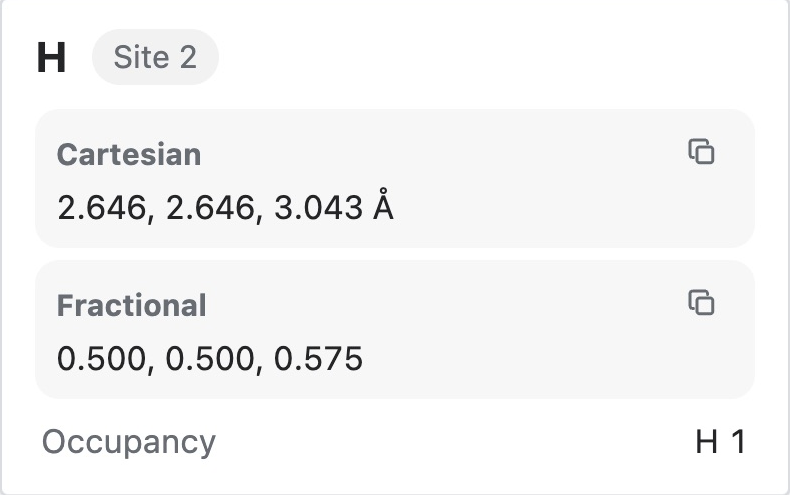
\includegraphics[width=79mm]{publication-assets/crop-f7556efd0d7de78b7cf1.png}
\caption{Online中初始氢分子第2个位点的坐标卡局部，显示笛卡尔坐标、分数坐标与占位。此时尚未改变初始几何；坐标卡用于核对读数，不是完整的模型视图。}
\label{fig:h2-structure-inspection}
\end{figure}

这一步既是检查，也是练习。电子结构计算对距离非常敏感，原子间距的小数点放错一位会得到完全不同的问题。对于本例，确认“两个氢原子、约 $0.794$ Å、约 $5.292$ Å 的立方盒”已经足够，无需逐项记住完整坐标。

如果使用自己的 XYZ 文件建立相同的氢分子，原子间距可以相同，模拟盒却未必相同。分子文件没有晶格时，软件会根据原子范围和真空距离构造盒子。要与本章数字作细致比较，应使用相同的模拟盒，而不仅是相同的键长。

\section{建立自洽计算工作流}

\subsection{从 SCF 模板开始}

工作流把计算过程分为若干节点。节点之间的连线表示处理顺序。本例只需要三项工作：把导入的结构交给求解器、计算电子结构、显示收敛过程。使用模板可以先得到这套基本关系，再逐项调整其中的参数。

\begin{steps}
\item 打开 \ui{工作流} 的导入菜单，选择 \ui{从模板建立工作流}。
\item 选择 \ui{SCF} 模板。
\item 打开新建的工作流文档，查看画布上的节点和连线。
\item 确认工作流包含结构配置、SCF 计算和能量曲线三个任务，并按这一顺序连接。图中的Online流程将结构配置节点标为\ui{Configuration}，随书桌面项目中同一任务标为\ui{Build Molecule}；后两个节点依次为\ui{SCF}和\ui{Plot}。
\end{steps}

若选择的是空白工作流，可以自行添加上述三个节点，再依次连接。节点的显示名称可以修改，任务类型则应保持正确。例如，把节点标签改为“计算氢分子”不会改变它是一个 SCF 任务。对于第一次操作，保留模板名称更容易与本章说明对应。

可以对照图\ref{fig:h2-workflow}检查顺序：第一个节点接收结构，第二个节点完成电子结构求解，最后一个节点读取计算历史并画出曲线。接下来按这个顺序逐项配置。

\begin{figure}[!htb]
\centering
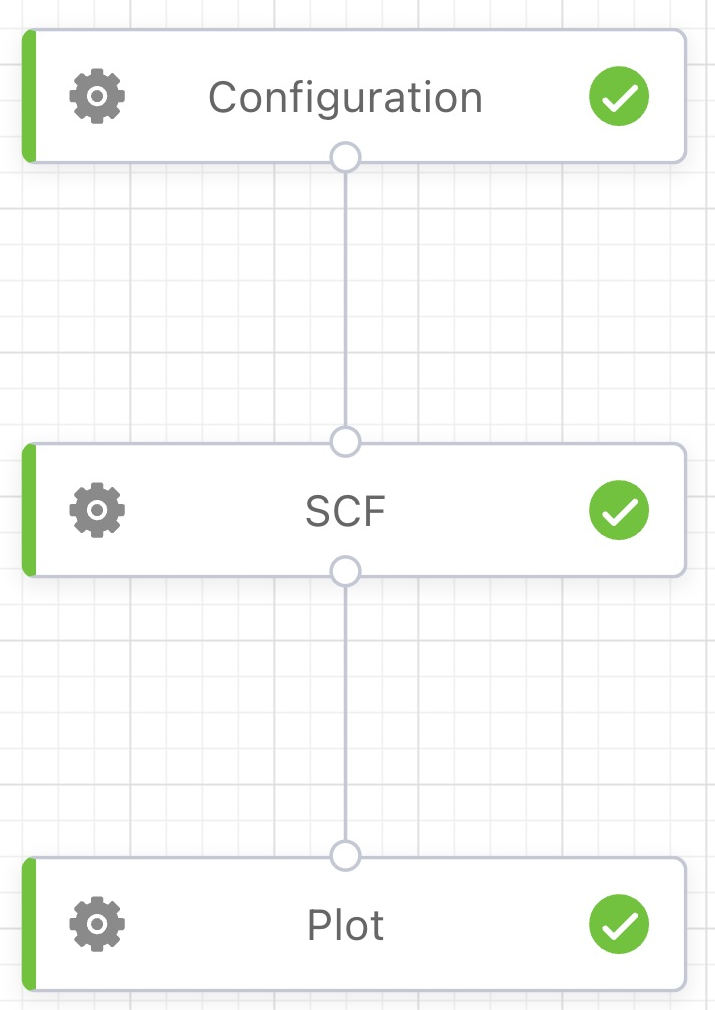
\includegraphics[width=60mm]{publication-assets/crop-273037e846506daab173.png}
\caption{本次Online氢分子计算完成后的SCF流程。结构配置、电子结构求解和绘制曲线自上而下连接；Configuration对应Build Molecule任务，Plot对应绘制收敛曲线。}
\label{fig:h2-workflow}
\end{figure}

\subsection{配置结构输入}

在画布上选择结构配置节点，本次Online中标为\ui{Configuration}，再选择 \ui{工作流 → 配置节点}，也可以使用节点上的齿轮。这项命令会展开原本收起的右侧面板，并在 \ui{配置编辑器} 中打开或刷新该节点的专用设置；向下滚动到 \ui{选项} 区，便可以看到 Type 等参数。只看到节点 ID、标签、模块等通用属性时，请先执行配置节点命令。这个节点既指定结构，也规定求解时采用的物理和数值模型。请不要只确认结构名称便直接运行；模板中可能保存着上一次制作模板时的参数。

如果面板较窄，参数名称或下拉框内容可能被截短。点击\ui{配置编辑器}标题栏右上角的省略号，选择\ui{最大化}，可以暂时把主要工作区让给这个面板。完成填写后，再从同一菜单选择\ui{还原}，回到画布与参数并列的布局。\ui{通用}、\ui{输入}、\ui{选项}和\ui{高级选项}各自可以展开或折叠；填写本例时，可先折叠通用与输入，把空间留给选项。

\begin{steps}
\item 将 \ui{Type} 设为 \ui{Molecule}。
\item 在 \ui{Choose imported structures} 中只选择本例的氢分子。
\item 将 \ui{Functional} 设为 \ui{PBE}，\ui{Pseudopotential} 设为 \ui{default}。
\item 在 \ui{Ecut (Hartree)} 中输入 \texttt{20}。
\item 保持 \ui{Smearing} 为 \ui{fermi-dirac}，\ui{Temperature (K)} 为 \texttt{0}，\ui{Nspin} 为 \texttt{1}。
\item 在高级选项中保持额外能带数为 \texttt{0}。
\end{steps}

选择 Molecule 后，晶体的自动 k 点设置不再是本例需要调整的内容。氢分子的这个计算使用盒内分子模式。不要为了与其他教程的晶体参数看起来一致而设置一张密集的 k 点网格。

\ui{Ecut (Hartree)} 中的单位尤其值得留意。这里输入 $20$ 表示 $20$ Ha，约合 $544$ eV；它并不是 $20$ eV。图形界面把单位写在标签里，阅读论文或其他软件的输入时，也应先完成单位换算，再比较参数大小。

\begin{figure}[H]
\centering
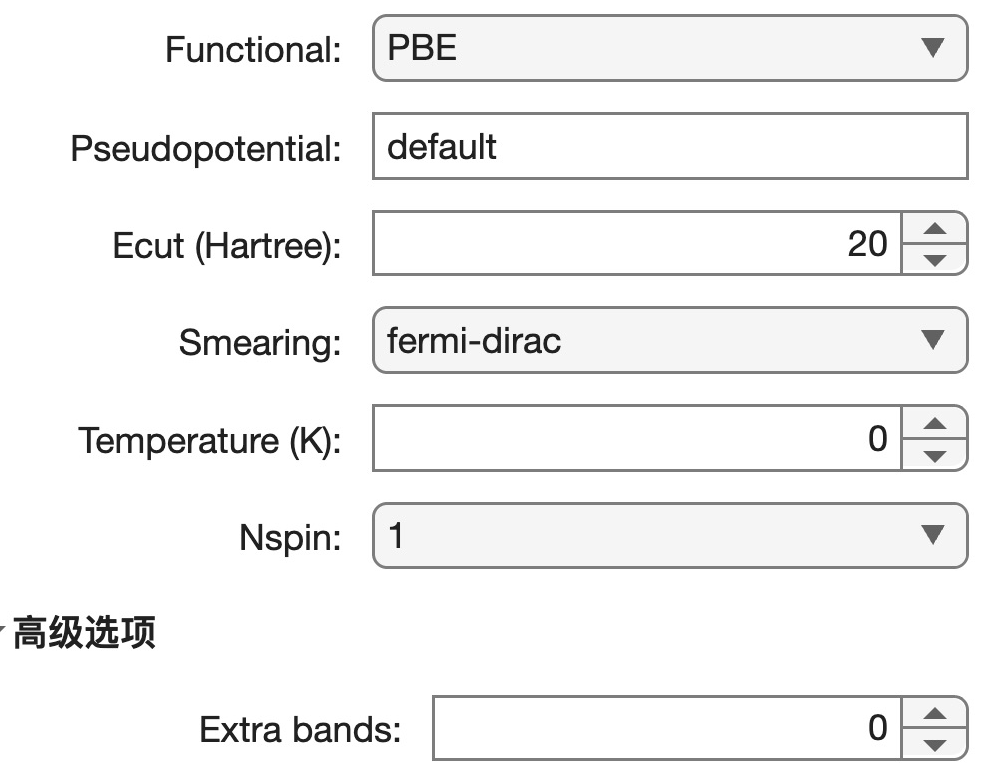
\includegraphics[width=90mm]{publication-assets/crop-1d148adc90da2955994e.png}
\caption{本次Online结构配置的常规与高级选项。PBE、default赝势、20 Ha、0 K、Nspin=1和Extra bands=0均可在此核对；Molecule与结构h2的选择见图\ref{fig:online-h2-config}。}
\label{fig:h2-build-options}
\end{figure}

\subsection{配置 SCF 节点}

选择 \ui{SCF} 节点，再选择 \ui{工作流 → 配置节点}，向下滚动到它的 \ui{选项} 区。\ui{DiagMethod} 决定每一步求解电子态时使用的数值方法；\ui{Max SCF steps} 则规定电子密度最多更新多少次。对于本例，使用默认的 \ui{davidson\_qe} 和 $100$ 步即可。

展开\ui{DiagMethod}下拉框时，可以看到多种方法。本例选择\ui{davidson\_qe}；收起后如果文字显示不全，可最大化面板核对完整名称。

\begin{figure}[!htb]
\centering
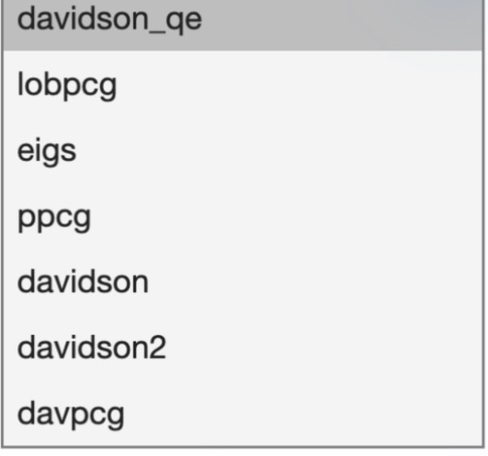
\includegraphics[width=48mm]{publication-assets/crop-1581def0867bec552a40.png}
\caption{Online中SCF节点的算法列表。本例使用davidson\_qe；其他方法保留给有明确比较目标的计算。}
\label{fig:h2-scf-methods}
\end{figure}

选中 \ui{Calculate force}。原子力表示在当前电子分布下，原子沿哪个方向移动会降低能量。本章先不移动原子，计算力是为了在后面的优化教程中比较起点和终点。若不需要原子力，普通单点能计算可以不勾选这一项。

高级选项中的 \ui{ExxMethod} 保持 \ui{default}。它主要服务于杂化泛函计算，不需要在本例的 PBE 计算中额外调整。

完成填写后，按表\ref{tab:h2-scf-options}逐项核对。较长的方法名可以在最大化的配置编辑器中阅读，核对后再还原布局。

\begin{table}[!htb]
\centering
\caption{氢分子教程的 SCF 节点参数}
\label{tab:h2-scf-options}
\begin{tabularx}{\linewidth}{lX}
\toprule
选项 & 本例设置\\
\midrule
\ui{DiagMethod} & \ui{davidson\_qe}，每一步求解电子态所用的方法\\
\ui{Max SCF steps} & \texttt{100}，电子密度更新的最大步数\\
\ui{Calculate force} & 选中，在本次单点计算中求原子力\\
\ui{ExxMethod} & \ui{default}，本例保持高级选项的默认设置\\
\bottomrule
\end{tabularx}
\end{table}

\subsection{检查曲线节点}

能量曲线任务负责把 SCF 的历史记录画成图，在本例画布上标为\ui{Plot}。它不再求一次电子结构，也不改变上一步的结果。确认它位于 SCF 之后即可。如果先运行 SCF，随后才添加曲线节点，可以再次执行这条完整的小工作流，得到与该次计算对应的曲线。

在运行前保存项目。以后比较不同截断能、不同结构或不同泛函时，保存的工作流便是说明计算条件最直接的记录。

\section{运行计算并观察进度}

\subsection{选择正确的工作流}

应用中可以同时打开多个工作流文档。运行之前，先点击本例工作流的文档标签，让它成为当前工作流，再选择 \ui{运行}。这样可以避免模型已经切换而运行的仍是另一张工作流的情况。

运行前展开右侧面板组，再展开\ui{模拟浏览器}的标题栏；如果面板已经关闭，可从\ui{打开面板}列表中按名称打开。配置编辑器仍占满工作区时，先用标题栏菜单\ui{还原}，便可同时观察画布和输出。运行后，这里开始显示计算消息。SCF 日志通常按迭代步依次列出误差、总能量和耗时。某一步的误差下降较慢，并不意味着操作有误；判断整个计算时，应查看完整的迭代过程和最终的收敛状态。

\begin{steps}
\item 使氢分子的 SCF 工作流处于当前文档。
\item 选择 \ui{主页 → 运行}，或使用模拟浏览器中的 \ui{运行} 按钮。
\item 在模拟浏览器中找到氢分子计算开始的消息。
\item 等待出现收敛消息，随后查看自动打开的曲线。
\item 返回工作流画布，确认需要执行的节点已经完成。
\end{steps}

本地\ui{停止}按钮目前只恢复运行按钮状态，不会中断正在进行的数值求解；Online同步计算也不提供停止操作。本例应等待计算结束后再继续。运行期间可查看日志判断进度，关闭浏览器标签不会保存项目或结束服务器计算。

\subsection{测量一次运行的用时}

\ui{运行}右侧的下拉菜单提供\ui{运行并计时}。需要做这个练习时，先激活本章SCF流程，再选择该项；本地流程完成后，窗口底部显示本次用时。计时包含这次流程的执行和相关准备，不是每个节点的独立性能分析。

比较用时之前，保持模型、参数和执行环境一致，并说明是否首次运行。首次打开数值功能或生成图形可能增加准备时间。使用远程配置提交作业时，本地提交耗时不等于远端计算耗时，应阅读远程作业的记录。保存本章项目时，可以将计时另记在实验笔记中，科学结果仍以能量、误差与收敛状态判断。


\subsection{理解日志中的三个数字}

第一次阅读日志时，先关注迭代编号、相对密度误差和总能量。迭代编号表明求解器进行了多少次更新；密度误差反映前后两次电子密度的差别；总能量则是当前密度下对体系能量的估计。

电子密度逐渐自洽时，总能量往往趋于稳定，但能量序列不一定严格单调。求解器会混合历史密度以加快收敛，因此某一步能量稍有回升仍可能是正常的数值过程。判断是否完成，应读最终的收敛信息，而不是只看最后两行能量是否相同。

\begin{figure}[!htb]
\centering
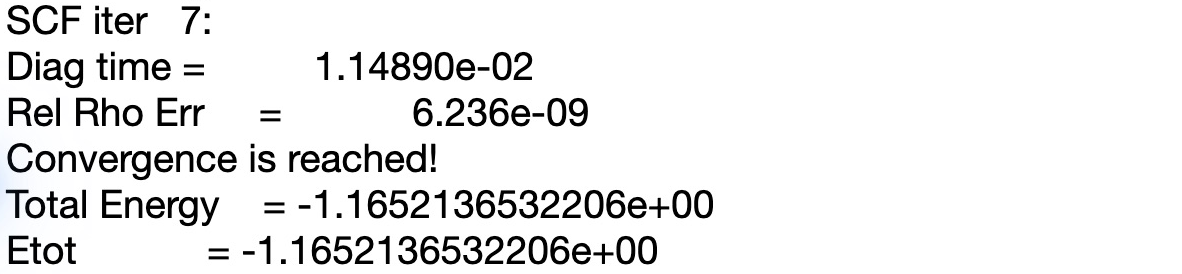
\includegraphics[width=119.9mm]{publication-assets/crop-2984400ea30d3f4eb1f5.png}
\caption{本次Online氢分子SCF运行的日志局部。第7步出现\ui{Convergence is reached!}，总能量为$-1.1652136532206$ Ha，相对密度误差约为$6.24\times10^{-9}$。}
\label{fig:h2-scf-runtime-log}
\end{figure}

\section{阅读第一幅计算结果}

\subsection{读懂收敛曲线}

收敛图把同一次 SCF 的两类记录画在一起。横轴是迭代次数，左纵轴为总能量，单位 Ha；右纵轴为误差。误差轴使用对数刻度，因此相同的纵向距离可以对应误差相差一个或多个数量级。

观察图形时，可以先沿着能量曲线从左往右阅读，再看误差是否整体降低。对于这个很小的氢分子，能量在开始几步便接近稳定，误差仍需进一步下降。这说明“图上看起来已经平了”和“求解器已经达到收敛条件”是两个不同的判断。

\begin{figure}[!htb]
\centering
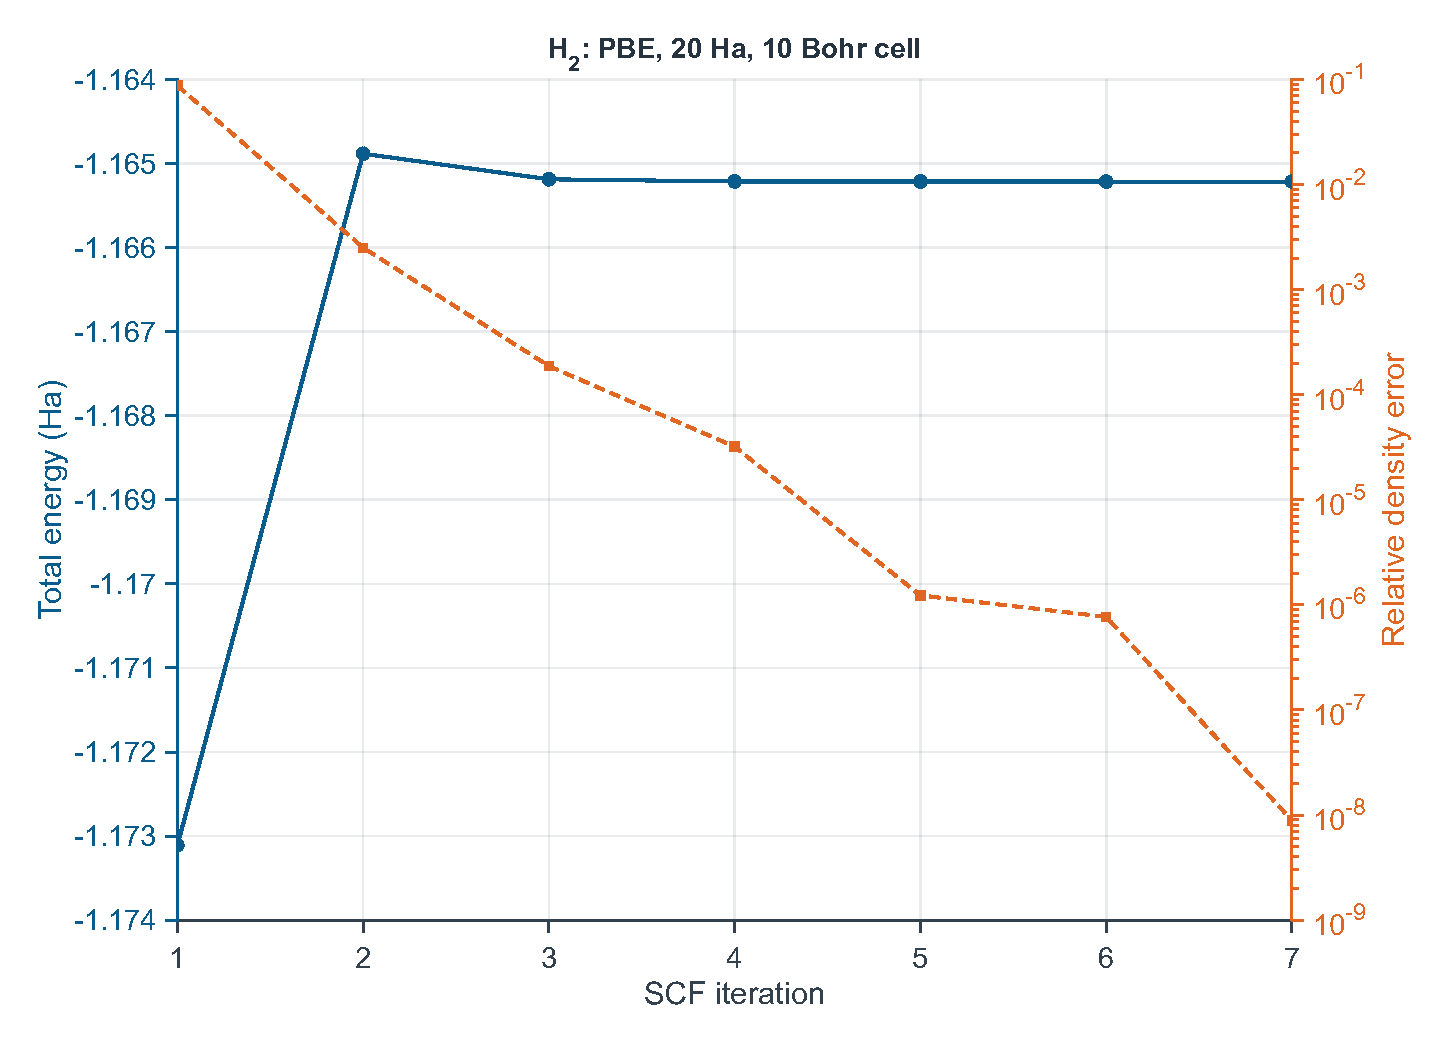
\includegraphics[width=\linewidth]{publication-assets/vector-2e572f3c8654292658e8.pdf}
\caption{氢分子自洽计算的总能量与相对密度误差。蓝线读左轴，橙色虚线读右侧对数轴；图中数据来自随书参考运行。}
\label{fig:h2-scf-results}
\end{figure}

\subsection{与本书的参考运行比较}

本书配套脚本在 macOS Apple Silicon、MATLAB R2026b 的无 JVM 批处理环境中完成了相同条件的 CPU 计算。固定随机种子后，SCF 在 $7$ 步达到收敛，总能量为约 $-1.1652136531$ Ha，最后的相对密度误差约为 $8.85\times10^{-9}$。这些数字来自保留的运行日志，作为识别教程输入是否一致的参照。

本次Online计算在7步后收敛，总能量约为$-1.1652136532$ Ha，相对密度误差约为$6.24\times10^{-9}$。它与随书脚本的总能量相差约$1.44\times10^{-10}$ Ha，两次计算均满足本例的收敛条件。图\ref{fig:h2-scf-results}仍采用随书脚本的数据绘制，便于在纸面上清楚阅读坐标和曲线。

在图形界面中运行时，初始电子态、软件版本和数值环境可能使迭代次数或最后几位数字略有不同。比较时先确认结构、盒尺寸、泛函、赝势和截断能一致，再检查最终是否收敛。一次计算的耗时受设备和会话负载影响，因此本教程不把完成秒数作为操作正确与否的标准。

\begin{notebox}{总能量的含义}
本例的总能量属于这个盒中、这个几何构型、这套泛函和赝势条件下的氢分子。它不直接等于实验中的分子结合能。若要计算解离能，还需要以一致的方法计算相应的原子参考态，并处理自旋等条件。
\end{notebox}

\subsection{保存结果和项目}

计算曲线加入项目的结果分类后，可以从项目浏览器再次打开。图形是计算记录的一种呈现，工作流保存的是产生它的步骤，两者都有保留的价值。建议在运行后再次保存项目，而不只是在运行前保存一次。

为图形使用容易理解的名称，例如“氢分子：PBE，20 Ha，初始结构”。如果后面还要计算优化后的结构，清楚的名称可以避免把两个构型的结果混在一起。名称中可以放主要条件，完整参数则留在工作流中，不必把所有内容塞进一个很长的文件名。

\section{完成本章练习}

重新打开保存的项目，确认结构、工作流中的结构选择和结果图都能恢复。

作为延伸练习，再次导入\file{h2.cif}，命名为\file{H2-longer}。按第~\ref{ch:modeling}~章的几何编辑方法，将键长设为$0.85\,\text{\AA}$；随后回到\ui{Build Molecule}，在\ui{Choose imported structures}中改选这一结构，保持截断能、泛函和模拟盒不变，再运行单点计算。分别保存两次结果，比较总能量和沿键方向的力。第~\ref{ch:workflows}~章继续介绍几何优化，第~\ref{ch:results}~章介绍结果解读。

\section{用脚本复现本例}

本节面向使用完整 MATLAB 的读者。独立应用和 Online 可以继续使用前面的图形操作，无需执行配套脚本。图形界面便于学习和检查结构，脚本便于重复执行相同参数。配套 \file{examples/h2_scf_and_relax.m} 给出完整输入；下面摘录其中的单点计算部分。此段代码用于已经初始化 KSSOLV 数值环境的 MATLAB 会话。

\Needspace{11\baselineskip}
\begin{lstlisting}[language=Matlab]
pseudopotential.PpType('default');
molecule = example.structure.H2();
molecule.ecut = 20;
molecule.funct = 'PBE';
scfOptions = options.SCF('force', true);
scfOptions.enableGPU = false;
scfOptions.enableParallelPool = false;
[molecule, H, X, info] = scf(molecule, scfOptions);
\end{lstlisting}

返回值中，\texttt{info.Etot}是总能量，\texttt{info.Etotvec}和\texttt{info.SCFerrvec}记录能量与误差历史，\texttt{info.converge}给出收敛状态，可用于整理表格或绘图。配套脚本还会继续优化原子位置并保存数据；只重复本章时，执行上述单点部分即可。图形界面与脚本采用同一数值模型，操作时沿用本例明确给出的参数。

